\chapter{Grundlagen des Deep Metric Learning}
\label{chap:grundlagen}


Dieses Kapitel stellt die Begriffe und die Verfahren bereit, auf denen die Versuche dieser Arbeit aufbauen. Es beginnt mit dem klassischen Metric Learning und dessen Erweiterung auf tiefe neuronale Netze (Abschnitte~\ref{sec:ml} und~\ref{sec:dml}). Danach folgen die Verlustfunktionen, mit denen Embeddings trainiert werden (Abschnitt~\ref{sec:verluste}). Abschnitt~\ref{sec:sampling} behandelt die Frage, welche Paare ein Batch enthalten sollte. Abschnitt~\ref{sec:bewertung} beschreibt, wie Retrieval-Ergebnisse bewertet werden, Abschnitt~\ref{sec:geometrie} führt Maße für die Geometrie eines Embedding-Raums ein. Den Abschluss bilden das vortrainierte Backbone DINOv2 (Abschnitt~\ref{sec:vit}) sowie faire Vergleiche, die Modellauswahl und die Hyperparameteroptimierung (Abschnitt~\ref{sec:modellauswahl}). 

\section{Metric Learning}
\label{sec:ml}

\emph{Metric-Learning}-Verfahren lernen eine Distanzfunktion aus Angaben darüber, welche Datenpunkte als ähnlich gelten und welche nicht~\cite{bellet_survey_2014}. Solche Distanzfunktionen kommen unter anderem bei der Klassifikation, beim Clustering und im Information Retrieval zum Einsatz~\cite{bellet_survey_2014}. Bei der $k$-Nearest-Neighbor-Klassifikation bestimmt etwa die Distanz, welche Nachbarn über die Klasse eines Beispiels abstimmen~\cite{bellet_survey_2014, weinberger_distance_2009}. Im Information Retrieval werden anhand der Ähnlichkeit zu einer Anfrage passende Ergebnisse gesucht und geordnet. Für diese Anwendungen ist die Wahl des Distanzmaßes entscheidend~\cite{bellet_survey_2014}. Die euklidische Distanz gewichtet alle Richtungen des Merkmalsraums gleich, auch wenn sie für die jeweilige Aufgabe unterschiedlich relevant sind~\cite{bellet_survey_2014, weinberger_distance_2009}.

Eine Funktion $d$ auf Paaren von Datenpunkten ist eine Metrik, wenn sie nichtnegativ und symmetrisch ist, die Dreiecksungleichung erfüllt und genau dann null wird, wenn beide Argumente gleich sind. Bei dem Metric Learning wird beispielsweise eine Mahalanobis-Distanz gelernt~\cite{bellet_survey_2014, weinberger_distance_2009}:
\begin{equation}
  d_{\bm{M}}(\bm{x}_i,\bm{x}_j)=\sqrt{(\bm{x}_i-\bm{x}_j)^{\top}\bm{M}\,(\bm{x}_i-\bm{x}_j)}
  =\lVert\bm{A}\bm{x}_i-\bm{A}\bm{x}_j\rVert_2,
  \qquad \bm{M}=\bm{A}^{\top}\bm{A}\succeq\bm{0}.
  \label{eq:mahalanobis}
\end{equation}
Dabei bezeichnet $\bm{M}\succeq\bm{0}$ eine positiv semidefinite Matrix. Eine Mahalanobis-Distanz entspricht damit der euklidischen Distanz nach der linearen Abbildung $\bm{A}$ und ist auf dem Eingaberaum genau bei vollem Spaltenrang von $\bm{A}$ eine Metrik~\cite{bellet_survey_2014, weinberger_distance_2009}.

Als Lernsignal dienen etwa Mengen ähnlicher Paare, Mengen unähnlicher Paare oder relative Angaben der Form \enquote{$\bm{x}_i$ ist $\bm{x}_p$ ähnlicher als $\bm{x}_n$}~\cite{bellet_survey_2014}. In dieser Arbeit gelten Paare derselben Klasse als ähnlich, die verschiedener Klassen als unähnlich. 

Ein frühes Verfahren des Metric Learning minimiert die Summe der quadrierten Distanzen ähnlicher Paare unter der Nebenbedingung, dass die Summe der Distanzen unähnlicher Paare mindestens eins beträgt~\cite{xing_distance_2002}. \ac{LMNN} formuliert das Ziel dagegen lokal, unter anderem mit einem Margenterm über Tripel aus einem Punkt, einem vorab festgelegten Nachbarn derselben Klasse und einem Punkt einer anderen Klasse, dessen quadrierte Distanz die des Nachbarn um eine Marge übersteigen soll~\cite{weinberger_distance_2009}. Der in Abschnitt~\ref{sec:verluste} beschriebene Triplet Loss aus dem \ac{DML} ist durch diese Formulierung motiviert~\cite{schroff_facenet_2015}. 


Da die klassischen Mahalanobis-basierten Verfahren an eine lineare Abbildung der Merkmale gebunden sind, genügen sie nicht, wenn sich die Klassen erst nach einer nichtlinearen Transformation gut trennen lassen. Kernel-Verfahren ermöglichen zwar das Lernen einer Metrik in einem nichtlinearen Merkmalsraum, skalieren aber schlecht mit der Anzahl der Trainingsbeispiele \cite{bellet_survey_2014}. Deep Metric Learning nutzt stattdessen neuronale Netze mit nichtlinearen Aktivierungsfunktionen~\cite{kaya_deep_2019}. 



\section{Deep Metric Learning und Retrieval}
\label{sec:dml}

Die Verbindung von Metric Learning mit tiefen neuronalen Netzen wird als \ac{DML} bezeichnet~\cite{musgrave_metric_2020}. Die lineare Abbildung wird dabei durch ein neuronales Netz $\Phi(\cdot;\bm{\theta})$ ersetzt. Das \emph{Embedding} eines Bildes $\bm{x}_i$ ist $\bm{z}_i=\Phi(\bm{x}_i;\bm{\theta})\in\mathbb{R}^{n_{\mathrm{D}}}$. Die Distanz zweier Bilder ist dann die Distanz ihrer Embeddings \cite{mohan_deep_2023, hadsell_dimensionality_2006}. Als Grundlage von $\Phi$ dient ein vortrainiertes \emph{Backbone}. In den Vergleichsstudien zum \ac{DML} sind das \acp{CNN} wie GoogLeNet, BN-Inception oder ResNet50~\cite{musgrave_metric_2020, roth_revisiting_2020}. Neuere Arbeiten zum \ac{DML} verwenden \acp{ViT} und übertreffen damit auf denselben Benchmarks die zuvor mit \acp{CNN} berichteten Ergebnisse. Die Vergleiche werden jedoch durch Unterschiede im Vortraining beeinflusst, da einige der verwendeten \acp{ViT} auf dem größeren ImageNet-21k statt auf ImageNet-1k vortrainiert  wurden \cite{ermolov_hyperbolic_2022, ren_learning_2024}. 
Bei der Festlegung von Grundeinstellungen für das Training von Retrieval-Modellen ging aus mehreren ResNets und den Größen S und B von DINOv2 das DINOv2-B als Backbone hervor. Dort wurden zudem Embeddings unterschiedlicher Dimension $n_{\mathrm{D}}$, die eine zusätzliche lineare Schicht erzeugt, mit den unveränderten Merkmalen des Backbones verglichen \cite{berton_all_2025}.
 Die Embeddings können auf Länge eins normiert werden~\cite{schroff_facenet_2015}:
\begin{equation}
	\bm{f}_i=\frac{\bm{z}_i}{\lVert\bm{z}_i\rVert_2},\qquad \lVert\bm{z}_i\rVert_2>0.
\end{equation}
Die normierten Embeddings $\bm{f}_i$ liegen damit auf der Einheitssphäre und ihre Kosinusähnlichkeit ist das Skalarprodukt $s_{ij}=\bm{f}_i^{\top}\bm{f}_j\in[-1,1]$. Wegen $\lVert\bm{f}_i-\bm{f}_j\rVert_2^2=2-2s_{ij}$ liegen ihre euklidischen Distanzen im Intervall $[0,2]$ und die Sortierung nach aufsteigender Distanz entspricht der nach absteigender Kosinusähnlichkeit.

Ob ein Modell Ähnlichkeiten auch zwischen bisher ungesehenen Klassen erkennt, lässt sich mit Trainings- und Testmengen prüfen, die keine Klasse gemeinsam haben~\cite{song_deep_2016}. Ein verbreitetes Evaluationsprotokoll teilt die Klassen dafür in zwei gleich große Mengen~\cite{musgrave_metric_2020, song_deep_2016}. Daraus folgt für diese Arbeit, dass ein guter Embedding-Raum auch Bilder unbekannter Klassen gruppieren muss. Bei fine-grained-Datensätzen muss das Modell Merkmale lernen, mit denen sich auch bisher ungesehene Klassen unterscheiden lassen, wie zum Beispiel die Form von Scheinwerfern oder den Verlauf von Nähten an Kleidungsstücken.

Eine typische Anwendung ist das in Kapitel~\ref{chap:einleitung} beschriebene Retrieval, bei dem die Bilder eingebettet und nach ihrer Distanz zur Query geordnet werden~\cite{musgrave_metric_2020}. Bei Cars196 und \ac{CUB} dient jedes Testbild als Query und wird mit allen übrigen Testbildern verglichen~\cite{song_deep_2016}. Bei dem In-Shop-Datensatz suchen die Querys dagegen nur in einer gemeinsamen, von ihnen getrennten Bildmenge, der \emph{Gallery}~\cite{wang_multi-similarity_2019, kim_proxy_2020}. Als relevant gelten Bilder derselben Klasse, bei dem In-Shop-Datensatz also Bilder desselben Kleidungsstücks~\cite{liu_deepfashion_2016}.

\section{Verlustfunktionen}
\label{sec:verluste}

Die Verlustfunktion steuert, welchen anderen Embeddings oder welchen Klassenrepräsentanten ein Embedding während des Trainings angenähert und von welchen es entfernt wird. Die hier zitierten Arbeiten verwenden unterschiedliche Bezeichnungen für die Gruppen von Verlustfunktionen. Zu den \emph{Embedding Losses} zählen etwa der Contrastive Loss, der Triplet Loss und der \ac{MS} Loss, zu den \emph{Classification Losses} der normierte Softmax-Verlust, CosFace und ArcFace~\cite{musgrave_metric_2020}. Daneben werden die Embedding Losses auch \emph{ranking-based} genannt und von den \emph{classification-based} und den \emph{proxy-based} Verfahren als zwei weiteren Gruppen unterschieden~\cite{roth_revisiting_2020}. Der Name verweist dort auf das Ziel, dass gleichklassige Bilder einem Anker näher liegen als Bilder fremder Klassen. Bei den proxy-based Verfahren vertreten dagegen mitgelernte Vektoren die Klassen im Embedding-Raum. Für ranking-based Verfahren wie den Contrastive Loss und den \ac{MS} Loss sind die Bezeichnungen \emph{Ranking Losses} und genauer \emph{pair-based ranking losses} zu finden~\cite{duan_slade_2021}. Auch die Bezeichnungen \emph{contrastive} und \emph{classification losses} kommen vor~\cite{berton_all_2025}. Schließlich werden die Verfahren auch in \emph{pair-based} und \emph{proxy-based} Formulierungen sowie Regularisierungen gegliedert \cite{mohan_deep_2023}.

Uneinheitlich ist damit vor allem die Stellung der proxybasierten Verfahren. So wird Proxy-NCA zu den Classification Losses gezählt~\cite{musgrave_metric_2020}. Die Einteilung dieser Arbeit folgt der Dreiteilung in ranking-, proxy- und classification-based Verfahren~\cite{roth_revisiting_2020}. Verlustfunktionen, die die Embeddings eines Batches direkt miteinander vergleichen, heißen hier \emph{paarbasiert}, solche mit lernbaren Proxys \emph{proxybasiert} und solche mit einem Klassifikator über alle Trainingsklassen \emph{klassifikationsbasiert}.

\begin{figure}[tbp]
  \centering
  \begin{tikzpicture}[diagram,
  pt/.append style={minimum size=2.2mm},
  pull/.style={->, line width=0.6pt, draw=tolblue, shorten <=1.2mm},
  push/.style={->, line width=0.6pt, draw=tolred, shorten <=1.2mm},
  neg2/.style={pt, fill=tolgreen},
  cproxy/.style={proxy, minimum size=2.4mm},
]
\begin{scope}[shift={(0,0)}]
\node[paneltitle] at (0,2.2) {(a) MS, Circle};
\node[anchorpt, minimum size=2.2mm] (A) at (1.7,0.9) {};
\node[pospt] (p1) at (2.6,1.5) {}; \node[pospt] (p2) at (0.8,1.55) {}; \node[pospt] (p3) at (2.85,0.45) {};
\node[negpt] (n1) at (1.3,0.45) {}; \node[negpt] (n2) at (2.1,0.2) {}; \node[neg2] (n3) at (0.45,0.6) {};
\draw[pull] (p1) -- ($(A)!0.45!(p1)$); \draw[pull] (p2) -- ($(A)!0.45!(p2)$);
\draw[pull, line width=1.2pt] (p3) -- ($(A)!0.45!(p3)$);
\draw[push, line width=1.2pt] (n1) -- ($(A)!2.0!(n1)$); \draw[push, line width=0.9pt] (n2) -- ($(A)!1.7!(n2)$);
\draw[push, line width=0.4pt, draw=tolgreen] (n3) -- ($(A)!1.3!(n3)$);
\end{scope}
\begin{scope}[shift={(3.95,0)}]
\node[paneltitle] at (0,2.2) {(b) NT-Xent};
\node[anchorpt, minimum size=2.2mm] (A) at (1.7,0.9) {};
\node[pospt] (p1) at ($(A)+(75:0.62)$) {};
\foreach \ang/\cc in {200/negpt,250/neg2,300/negpt,160/neg2,20/negpt,330/neg2,125/negpt} {\node[\cc] (x\ang) at ($(A)+(\ang:0.78)$) {};}
\draw[pull] (p1) -- ($(A)!0.4!(p1)$);
\foreach \ang/\cc in {200/tolred,250/tolgreen,300/tolred,160/tolgreen,20/tolred,330/tolgreen,125/tolred} {\draw[push, line width=0.45pt, draw=\cc] (x\ang) -- ($(A)!1.45!(x\ang)$);}
\end{scope}
\begin{scope}[shift={(7.9,0)}]
\node[paneltitle] at (0,2.2) {(c) Proxy-Anchor};
\node[cproxy, fill=black] (P) at (1.65,0.95) {};
\node[pospt] (b1) at (0.4,1.6) {}; \node[pospt] (b2) at (2.45,1.7) {}; \node[pospt] (b3) at (1.05,0.6) {};
\node[negpt] (n1) at (2.2,0.45) {}; \node[negpt] (n2) at (3.0,1.15) {}; \node[neg2] (n3) at (0.25,0.55) {};
\draw[pull, line width=1.2pt] (b1) -- ($(P)!0.3!(b1)$);
\draw[pull, line width=0.8pt] (b2) -- ($(P)!0.3!(b2)$);
\draw[pull, line width=0.5pt] (b3) -- ($(P)!0.3!(b3)$);
\draw[push, line width=1.2pt] (n1) -- ($(P)!1.7!(n1)$);
\draw[push, line width=0.5pt] (n2) -- ($(P)!1.35!(n2)$);
\draw[push, line width=0.5pt, draw=tolgreen] (n3) -- ($(P)!1.3!(n3)$);
\end{scope}
\begin{scope}[shift={(11.85,0)}]
\node[paneltitle] at (0,2.2) {(d) ArcFace};
\coordinate (O) at (0.9,0.15);
\draw[line width=0.4pt] ($(O)+(0:1.55)$) arc (0:125:1.55);
\draw[->, line width=0.6pt, draw=tolblue] (O) -- ($(O)+(30:1.55)$) node[anchor=south west, inner sep=1pt] {$\bm{w}_{y_i}$};
\draw[->, line width=0.6pt, draw=tolred] (O) -- ($(O)+(115:1.55)$) node[anchor=south east, inner sep=1pt] {$\bm{w}_{c}$};
\draw[->, line width=0.6pt] (O) -- ($(O)+(62:1.55)$) node[anchor=south, inner sep=1pt] {$\bm{f}_i$};
\draw[line width=0.4pt] ($(O)+(30:0.85)$) arc (30:62:0.85); \node at ($(O)+(45.5:1.17)$) {$\vartheta_{iy_i}$};
\draw[line width=0.5pt, dash pattern=on 2pt off 1.5pt] ($(O)+(62:0.85)$) arc (62:84:0.85); \node at ($(O)+(74:1.1)$) {$m$};
\end{scope}
\end{tikzpicture}

  \caption[Familien der verwendeten Verlustfunktionen]{Schematische Wirkung der fünf verwendeten Verlustfunktionen auf ein Bild (schwarzer Punkt). Blau: gleiche Klasse, rot und grün: andere Klassen, Quadrate: lernbare Klassenrepräsentanten (Proxys), Pfeile: Anziehung und Abstoßung, dick: stärker gewichtet. (a)~\acs{MS} Loss~\cite{wang_multi-similarity_2019} und Circle Loss~\cite{sun_circle_2020}, (b)~\acs{NT-Xent}~\cite{chen_simple_2020}, (c)~Proxy-Anchor~\cite{kim_proxy_2020}, (d)~ArcFace~\cite{deng_arcface_2018}. Darstellungsweise nach~\cite{kaya_deep_2019, kim_proxy_2020}.}
  \label{fig:verluste}
\end{figure}

Abbildung~\ref{fig:verluste} stellt die Wirkung der Familien auf ein einzelnes Bild dar. In den folgenden Formeln bezeichnet $\mathcal{B}$ die Indexmenge eines Batches der Größe $B$. Für einen Anker $i\in\mathcal{B}$ sind $\mathcal{P}_i=\{j\in\mathcal{B}\setminus\{i\}:y_j=y_i\}$ und $\mathcal{N}_i=\{j\in\mathcal{B}:y_j\ne y_i\}$ die Indizes der positiven bzw.\ negativen Bilder. Die Bezeichnungen $d_{ij}=\lVert\bm{f}_i-\bm{f}_j\rVert_2$ für die euklidische Distanz und $s_{ij}$ für die Kosinusähnlichkeit aus Abschnitt~\ref{sec:dml} gelten durchgehend. Die Klassenparameter und die Klassensummen beziehen sich auf die bekannten Klassen $\mathcal{C}_{\mathrm{L}}$ mit $C_{\mathrm{L}}=|\mathcal{C}_{\mathrm{L}}|$. Sind alle $C$ Trainingsklassen durch Labels vertreten, gilt $C_{\mathrm{L}}=C$ (Kapitel~\ref{chap:ssdml}). Margen $m$ und Skalen $\gamma$ werden für jede Verlustfunktion gesondert gewählt. Die Marge wirkt je nach Verlustfunktion auf Distanzen, Ähnlichkeiten oder Winkel. Der positive Teil ist $[\cdot]_+=\max\{0,\cdot\}$.

\subsection{Paarbasierte Verlustfunktionen}
\label{sec:verluste:paare}

Der \emph{Contrastive Loss} bewertet jedes Paar einzeln, mit einem Term für ähnliche und einem durch eine Marge begrenzten Term für unähnliche Paare. Für ähnliche Paare wächst der Verlust quadratisch mit dem Abstand. Für unähnliche Paare wird dagegen die quadrierte Differenz zwischen der Marge \(m\) und dem Abstand verwendet. Durch die Begrenzung auf nichtnegative Werte bleibt der Verlustterm für unähnliche Paare ab einem Abstand von $m$ gleich null \cite{hadsell_dimensionality_2006}. Diese Arbeit verwendet wie die Vergleichsstudie die Form mit getrennten Margen $m^{+}$ und $m^{-}$ für positive und negative Paare~\cite{musgrave_metric_2020},
\begin{equation}
  \mathcal{L}_{\mathrm{Contr},ij}=\begin{cases}[d_{ij}-m^{+}]_{+}, & j\in\mathcal{P}_i,\\ [m^{-}-d_{ij}]_{+}, & j\in\mathcal{N}_i.\end{cases}
  \label{eq:contrastive}
\end{equation}
 In Gleichung~\eqref{eq:contrastive} verschwindet der Term eines ähnlichen Paares mit $m^{+}=0$ erst bei $d_{ij}=0$, mit $m^{+}>0$ schon ab $d_{ij}\le m^{+}$ \cite{hadsell_dimensionality_2006}.

Der \emph{Triplet Loss} verlangt dagegen nur eine relative Abstandsbedingung. Für einen Anker $i$, ein positives Bild $p\in\mathcal{P}_i$ und ein negatives Bild $n\in\mathcal{N}_i$ soll die quadrierte Distanz zum negativen Bild um mindestens die Marge $m$ größer sein als die zum positiven Bild. FaceNet verwendet hierfür die quadrierten euklidischen Distanzen~\cite{schroff_facenet_2015}. Diese Arbeit verwendet wie beim Contrastive Loss diese Form mit einfachen Distanzen~\cite{musgrave_metric_2020},
\begin{equation}
  \mathcal{L}_{\mathrm{Triplet},ipn}=\bigl[d_{ip}-d_{in}+m\bigr]_{+}.
  \label{eq:triplet}
\end{equation}
Die Anzahl möglicher Tripel liegt bei $N$ Bildern in
$\mathcal{O}(N^3)$. Nach Gleichung~\eqref{eq:triplet} ist der Verlust null, sobald die Margenbedingung erfüllt ist. Solche Tripel tragen daher nicht zum Gradienten bei. FaceNet wählt deshalb gezielt Tripel aus, bei denen die Margenbedingung noch verletzt ist \cite{schroff_facenet_2015} (siehe Abschnitt~\ref{sec:sampling}).

Der \emph{\ac{MS} Loss} verbindet das Mining informativer Paare mit einer Gewichtung~\cite{wang_multi-similarity_2019}. 
Das Verfahren unterscheidet drei Arten von Ähnlichkeit. Die Selbstähnlichkeit $s_{ij}$ beschreibt die Kosinusähnlichkeit der beiden Embeddings eines Paares $(i,j)$. Hinzu kommen zwei relative Ähnlichkeiten, die das Paar mit anderen Paaren desselben Ankers $i$ vergleichen. Für ein negatives Paar wird die positive relative Ähnlichkeit anhand der Werte $s_{ip}$ mit $p\in\mathcal{P}_i$ bestimmt. Die negative relative Ähnlichkeit berücksichtigt dagegen die übrigen negativen Paare mit $n\in\mathcal{N}_i\setminus\{j\}$. Ein positives Paar wird entsprechend mit den negativen Paaren und mit den übrigen positiven Paaren desselben Ankers verglichen.
 Für das Mining zählt allein der Vergleich zwischen positiven und negativen Paaren, die positive relative Ähnlichkeit. Ein negatives Paar bleibt nur, wenn es ähnlicher ist als das unähnlichste positive Paar desselben Ankers abzüglich einer kleinen Marge $m_{\mathrm{Miner}}$, also $s_{ij}>\min_{p\in\mathcal{P}_i}s_{ip}-m_{\mathrm{Miner}}$. Ein positives Paar bleibt nur, wenn es unähnlicher ist als das ähnlichste negative Paar plus $m_{\mathrm{Miner}}$, also $s_{ij}<\max_{n\in\mathcal{N}_i}s_{in}+m_{\mathrm{Miner}}$. Die verbliebenen Paare mit den Indizes $\tilde{\mathcal{P}}_i\subseteq\mathcal{P}_i$ und $\tilde{\mathcal{N}}_i\subseteq\mathcal{N}_i$ gehen in die folgende Verlustfunktion ein. Ihr Gradient gewichtet ein negatives Paar umso stärker, je höher $s_{ij}$ ist und je weiter es die übrigen negativen Paare desselben Ankers darin übertrifft, ein positives Paar entsprechend umgekehrt~\cite{wang_multi-similarity_2019}. Der Beitrag eines Ankers $i$ zur Verlustfunktion lautet
\begin{equation}
  \mathcal{L}_{\mathrm{MS},i}=\frac{1}{\gamma^{+}}\log\Bigl[1+\sum_{p\in\tilde{\mathcal{P}}_i}\exp(-\gamma^{+}(s_{ip}-m))\Bigr]+\frac{1}{\gamma^{-}}\log\Bigl[1+\sum_{n\in\tilde{\mathcal{N}}_i}\exp(\gamma^{-}(s_{in}-m))\Bigr].
  \label{eq:ms}
\end{equation}
Logarithmen über Summen von Exponentialfunktionen sind geglättete Maxima~\cite{musgrave_metric_2020}. Aus Gleichung~\eqref{eq:ms} folgt damit, dass große Werte der Skalen $\gamma^{+}$ und $\gamma^{-}$ das Gewicht auf die schwierigsten positiven bzw.\ negativen Paare konzentrieren. Die Marge $m$ dient dabei als Referenzwert für die Ähnlichkeiten, gegenüber dem positive Paare mit niedriger und negative Paare mit hoher Ähnlichkeit stärker gewichtet werden~\cite{wang_multi-similarity_2019}.

In vielen auf Kosinusähnlichkeiten formulierten Verlustfunktionen gehen die Ähnlichkeiten eines positiven und eines negativen Paares über ihre Differenz ein. Mit den selbstgesteuerten Gewichten $w^{+}_{ij}=[1+m-\operatorname{sg}(s_{ij})]_+$ und $w^{-}_{ij}=[\operatorname{sg}(s_{ij})+m]_+$ und den vereinfachten Margen der Originalarbeit lautet der \emph{Circle Loss} in der Notation dieser Arbeit \cite{sun_circle_2020}
\begin{equation}
  \mathcal{L}_{\mathrm{Circle},i}=\log\Bigl[1+\sum_{p\in\mathcal{P}_i}\exp\bigl(-\gamma\,w^{+}_{ip}(s_{ip}-1+m)\bigr)\sum_{n\in\mathcal{N}_i}\exp\bigl(\gamma\,w^{-}_{in}(s_{in}-m)\bigr)\Bigr].
  \label{eq:circle}
\end{equation}
Dabei ist $\gamma$ eine Skala, $m$ die Marge und $\operatorname{sg}$ die Identität im Vorwärtslauf, deren Ableitung bei der Backpropagation null gesetzt wird \cite{sun_circle_2020}. Wie in der verwendeten Implementierung bleiben die Gewichte damit beim Differenzieren konstant~\cite{musgrave_pytorch_losses_code_2026}. Nach seiner Definition wächst $w^{+}_{ij}$ linear, je weiter $s_{ij}$ unter $1+m$ liegt. Entsprechend wächst $w^{-}_{ij}$ oberhalb von $-m$ und ist darunter null. Weniger gut optimierte Ähnlichkeiten tragen dadurch stärker zum Gradienten bei als bei einem Verlust über diese Differenz, der beide gleich behandelt~\cite{sun_circle_2020}.

\subsection{Softmax über viele Negative}
\label{sec:verluste:ntxent}

Der N-Pair Loss zieht je Klasse genau ein positives Bildpaar in den Batch~\cite{sohn_improved_2016}. Als Negativbeispiele eines Ankers dienen dort die zweiten Bilder der Paare aller anderen Klassen. Die Verlustfunktion wird auch InfoNCE oder \ac{NT-Xent} genannt~\cite{musgrave_metric_2020}. InfoNCE stammt aus dem kontrastiven Repräsentationslernen~\cite{oord_representation_2018}, der Name \ac{NT-Xent} aus dem Self-supervised Learning~\cite{chen_simple_2020}. Beim N-Pair Loss bleiben die Skalarprodukte dabei unnormiert und ihre Größe begrenzt nur eine Strafe auf die Norm der Embeddings~\cite{sohn_improved_2016}, bei \ac{NT-Xent} werden dagegen Kosinusähnlichkeiten durch eine Temperatur $\tau$ geteilt~\cite{chen_simple_2020}. In der verwendeten Implementierung erhält jedes positive Paar einen eigenen Verlustterm, in dessen Nenner neben dem Paar selbst die negativen Paare seines Ankers stehen~\cite{musgrave_pytorch_losses_code_2026}:
\begin{equation}
  \mathcal{L}_{\mathrm{NT\text{-}Xent},ip}=-\log\frac{\exp(s_{ip}/\tau)}{\exp(s_{ip}/\tau)+\sum_{n\in\mathcal{N}_i}\exp(s_{in}/\tau)},\qquad p\in\mathcal{P}_i.
  \label{eq:ntxent}
\end{equation}
Weil jedes Negative mit seinem Softmax-Anteil in den Gradienten eingeht, bestimmt $\tau$, wie stark sich das Lernsignal auf die ähnlichsten, also härtesten Negativen konzentriert~\cite{chen_simple_2020}. 

\subsection{Proxy- und klassifikationsbasierte Verlustfunktionen}
\label{sec:verluste:proxy}

Der Trainingsaufwand paarbasierter Verlustfunktionen kann quadratisch oder kubisch mit der Zahl $N$ der Trainingsbilder wachsen~\cite{kim_proxy_2020}. Proxybasierte Verlustfunktionen vergleichen daher jedes Bild nur mit wenigen mitgelernten Stellvertretern im Embedding-Raum, den Proxys~\cite{movshovitz-attias_no_2017, kim_proxy_2020}. Mit einem Proxy je Klasse und $C$ Klassen wächst der Aufwand dann nur mit $\mathcal{O}(NC)$~\cite{kim_proxy_2020}. Proxy-NCA vergleicht jedes Bild über exponentiell gewichtete negative Distanzen mit seinem positiven Proxy und den Proxys der anderen Klassen~\cite{movshovitz-attias_no_2017}. Der Gradient eines Bildes hängt dabei nur von den Proxys ab, nicht von den übrigen Bildern des Batches \cite{kim_proxy_2020}. Bei \emph{Proxy-Anchor} läuft deshalb die äußere Summe über die Proxys und die innere über die Bilder des Batches. In der Notation dieser Arbeit lautet der Verlust \cite{kim_proxy_2020}
\begin{equation}
  \mathcal{L}_{\mathrm{PA}}=\frac{1}{|\mathcal{C}_{\mathcal{B}}|}\sum_{c\in\mathcal{C}_{\mathcal{B}}}\log\Bigl(1+\sum_{i\in\mathcal{P}_c}\exp(-\gamma(s_{ic}-m))\Bigr)+\frac{1}{C_{\mathrm{L}}}\sum_{c\in\mathcal{C}_{\mathrm{L}}}\log\Bigl(1+\sum_{i\in\mathcal{N}_c}\exp(\gamma(s_{ic}+m))\Bigr).
  \label{eq:proxyanchor}
\end{equation}
Dabei ist $\bm{w}_c$ der normierte Proxy der Klasse $c$ und $s_{ic}=\bm{w}_c^{\top}\bm{f}_i$ seine Kosinusähnlichkeit zu Bild $i$. Die Menge $\mathcal{C}_{\mathcal{B}}$ enthält die Klassen, die im Batch vorkommen. Die Mengen $\mathcal{P}_c=\{i\in\mathcal{B}:y_i=c\}$ und $\mathcal{N}_c=\{i\in\mathcal{B}:y_i\ne c\}$ enthalten die Indizes der Bilder dieser Klasse bzw.\ der übrigen Klassen. Dabei ist $\gamma$ eine Skala und $m$ eine Marge. 
Da $\mathcal{P}_c$ und $\mathcal{N}_c$ für jeden Proxy getrennt betrachtet werden, hängt der Gradientenbeitrag eines Bildes von seiner Ähnlichkeit zum Proxy und von der Ähnlichkeit der übrigen Bilder derselben Gruppe zu ihm ab \cite{kim_proxy_2020}.


Werden Embeddings und Klassengewichte dabei auf Länge eins normiert, ist jedes Logit als Skalarprodukt zweier Einheitsvektoren die Kosinusähnlichkeit zwischen dem Embedding und dem Gewichtsvektor der Klasse. Weil diese Logits nur zwischen $-1$ und $1$ liegen, ist die Softmax-Wahrscheinlichkeit der richtigen Klasse bei $C_{\mathrm{L}}$ bekannten Klassen höchstens $\e/(\e+(C_{\mathrm{L}}-1)\,\e^{-1})$. Normierte Klassifikationsverluste multiplizieren die Logits deshalb mit einer Skala $\gamma$, die diese Grenze aufhebt~\cite{wang_normface_2017}. Für \ac{NT-Xent} folgt daraus, dass $1/\tau$ dieser Skala entspricht, denn auch dort gehen Kosinusähnlichkeiten aus $[-1,1]$ in die Softmax ein. Für $\tau=1$ ist die Wahrscheinlichkeit des positiven Paares in Gleichung~\eqref{eq:ntxent} höchstens $\e/(\e+|\mathcal{N}_i|\,\e^{-1})$. CosFace zieht vom Kosinus der richtigen Klasse eine additive Marge ab~\cite{wang_cosface_2018}. \emph{ArcFace} addiert die Marge stattdessen zum Winkel, in der Notation dieser Arbeit~\cite{deng_arcface_2018}:
\begin{equation}
  \mathcal{L}_{\mathrm{ArcFace},i}=-\log\frac{\exp(\gamma\cos(\vartheta_{iy_i}+m))}{\exp(\gamma\cos(\vartheta_{iy_i}+m))+\sum_{c\in\mathcal{C}_{\mathrm{L}}\setminus\{y_i\}}\exp(\gamma\cos\vartheta_{ic})},\qquad \cos\vartheta_{ic}=s_{ic},
  \label{eq:arcface}
\end{equation}
mit normierten Klassengewichten $\bm{w}_c$, die getrennt von den Gewichten des Projection Heads gelernt werden. Die verwendete Implementierung ersetzt für $\vartheta_{iy_i}>\pi-m$ den Zielkosinus $\cos(\vartheta_{iy_i}+m)$ durch $\cos\vartheta_{iy_i}-m\sin m$, damit das Ziel-Logit über den ganzen Winkelbereich monoton fällt~\cite{musgrave_pytorch_losses_code_2026}. Die Marge verschiebt die Entscheidungsgrenze, sodass ein Embedding erst dann auf der richtigen Seite liegt, wenn $\vartheta_{iy_i}$ um mindestens $m$ kleiner ist als der Winkel zu jedem anderen Klassengewicht~\cite{deng_arcface_2018}. Unter einheitlichen Versuchsbedingungen auf \ac{CUB}, Cars196 und Stanford Online Products liefern CosFace und ArcFace ähnliche Retrieval-Ergebnisse~\cite{musgrave_metric_2020}.

Für die semi-supervised Verfahren dieser Arbeit ist eine Eigenschaft der klassifikationsbasierten Verlustfunktionen entscheidend. Eine klassifikationsbasierte Verlustfunktion braucht für jedes Bild eine feste Spalte der Gewichtsmatrix~\cite{musgrave_metric_2020}, während einer paarbasierten die Angabe genügt, welche Bilder eines Batches zusammengehören~\cite{berton_all_2025}. In dieser Arbeit heißt das, dass ein Bild nur dann in einen proxy- oder klassifikationsbasierten Verlust eingehen kann, wenn ihm eine der gelabelten Trainingsklassen zugeordnet ist. Pseudo-Labels müssen deshalb eine bekannte Klasse treffen und Beziehungen zwischen ungelabelten Bildern ohne Klassenzuordnung, etwa ein als ähnlich eingestuftes Paar, lassen sich nicht direkt verarbeiten. Kapitel~\ref{chap:methodik} kommt bei der Umsetzung von \ac{SLADE} darauf zurück.

\section{Mining und Sampling}
\label{sec:sampling}

Paarbasierte Verlustfunktionen können nur Paare auswerten,
die innerhalb eines Batches entstehen~\cite{musgrave_metric_2020}.
Welche Paare das sind, hängt von zwei Schritten ab.
Das \emph{Sampling} bestimmt, welche Bilder überhaupt in einen
Batch gelangen~\cite{roth_revisiting_2020, musgrave_pytorch_losses_code_2026}.
Welche der im Batch möglichen Paare oder Tripel tatsächlich in die
Verlustberechnung eingehen, bestimmt das \emph{Online-Mining}~\cite{musgrave_metric_2020,musgrave_pytorch_losses_code_2026}.

Beim \emph{Samples-per-Class}-Sampling (\acsu{SPC}) legt
der Parameter $n_{\mathrm{S}}$ fest, wie viele Bilder jede
ausgewählte Klasse zu einem Batch beiträgt. Ein Batch der Größe $B$ besteht bei \ac{SPC}-$n_{\mathrm{S}}$ aus $B/n_{\mathrm{S}}$ zufällig gewählten Klassen mit je $n_{\mathrm{S}}$ zufälligen Bildern \cite{musgrave_metric_2020, roth_revisiting_2020}. \ac{SPC}-4 gilt als die in der Literatur übliche Wahl~\cite{roth_revisiting_2020}. Für Classification Losses wird auch \ac{SPC}-1 verwendet~\cite{musgrave_metric_2020}. \ac{SPC}-1 kommt hier nur für klassifikationsbasierte Verlustfunktionen in Frage, denn ohne ein zweites Bild derselben Klasse fehlen paarbasierten die positiven Paare~\cite{musgrave_metric_2020, berton_all_2025}. Für die Nutzung von \ac{SPC}-2 spricht, dass es bei einer
Auswertung von sechs Verlustfunktionen auf drei
Datensätzen konsistent besser als \ac{SPC}-4 abschnitt.
Die Unterschiede in der mittleren normierten Leistung
zwischen den Samplingstrategien betrugen dabei
bis zu 1,5\,\%~\cite{roth_revisiting_2020}. Die Ergebnisse liefern damit keinen eindeutigen Grund,
einfache SPC-Samplingstrategien grundsätzlich durch beispielsweise embeddingbasierte Verfahren \cite{roth_revisiting_2020} zu ersetzen.

Beim Online-Mining unterscheiden sich die Strategien
darin, welche Paare oder Tripel eines Batches sie verwenden. Es können beispielsweise alle, nur die härtesten Positiven und Negativen
oder semi-harte Negative verwendet werden \cite{musgrave_metric_2020,schroff_facenet_2015}. Dieses Mining lässt sich auch als Grenzfall der Gewichtung auffassen, bei dem ein verworfenes Paar nichts zum Gradienten beiträgt. Beim \ac{MS} Loss aus Abschnitt~\ref{sec:verluste:paare} legt der Miner fest, welche Paare anschließend gewichtet werden \cite{wang_multi-similarity_2019}.

\section{Bewertung von Retrieval-Ergebnissen}
\label{sec:bewertung}

Retrieval-Metriken bewerten die Rangfolge der nächsten
Nachbarn eines Anfragebildes. Sie unterscheiden sich darin,
welche Positionen des Rankings sie
berücksichtigen. In der DML-Literatur wird häufig
Recall@$K$ berichtet, ergänzt durch Clustering-Metriken
wie \ac{NMI} und F1~\cite{musgrave_metric_2020}. Eine Query gilt bei Recall@$K$ als erfolgreich,
wenn unter den ersten $K$ Treffern mindestens
ein Bild derselben Klasse gefunden wird.
Die Metrik gibt den Anteil erfolgreicher
Querys an~\cite{song_deep_2016}. Recall@$K$ berücksichtigt damit nicht, wie viele
weitere relevante Bilder gefunden werden.
Ein konstruiertes Beispiel in
\textcite{musgrave_metric_2020}
zeigt drei Embedding-Räume mit unterschiedlich
gut getrennten Klassen. Trotz dieser Unterschiede
liegen die Recall@1-Werte zwischen \num{99} und
\num{100}\,\% und die NMI-Werte zwischen
\num{95.6} und \num{100}\,\%.

Als Alternative wird dort deshalb \ac{MAP@R} vorgeschlagen, das die Rangfolge der ersten Treffer bewertet. Ihre Zahl entspricht der Zahl der relevanten Bilder einer Query. Für eine Query $q$ mit mindestens einem relevanten Bild sei $R_q>0$ die Zahl der übrigen Bilder derselben Klasse in der durchsuchten Menge und $\operatorname{rel}_q(r)$ die Relevanz des Treffers auf Rang~$r$, also eins für einen Treffer aus der Klasse der Query und sonst null. In dieser Notation gilt~\cite{musgrave_metric_2020}
\begin{equation}
  \begin{gathered}
  \mathrm{P@1}_q=\operatorname{rel}_q(1),\qquad
  \mathrm{RP}_q=\frac{1}{R_q}\sum_{r=1}^{R_q}\operatorname{rel}_q(r),\\
  \mathrm{AP@R}_q=\frac{1}{R_q}\sum_{r=1}^{R_q}\operatorname{rel}_q(r)\,\frac{1}{r}\sum_{r'=1}^{r}\operatorname{rel}_q(r').
  \end{gathered}
  \label{eq:mapr}
\end{equation}
Dabei gibt die R-Precision (RP) an, welcher Anteil
der ersten $R_q$ Treffer relevant ist.
MAP@R mittelt die Werte $\mathrm{AP@R}_q$ über alle Querys
und berücksichtigt damit ebenfalls nur die ersten
$R_q$ Ränge. Jeder relevante Treffer geht mit der
Präzision bis zu seinem Rang in die Berechnung ein,
während irrelevante Treffer keinen direkten
Summanden beitragen.
Nach Gleichung~\eqref{eq:mapr} hängt $\mathrm{AP@R}_q$ davon ab, auf
welchem der ersten $R_q$ Ränge ein
relevanter Treffer steht. Bei $R_q=2$ und einem relevanten Treffer
ergibt Rang~1 ein $\mathrm{AP@R}_q$ von \num{0.5}, Rang~2 nur \num{0.25}, während die
R-Precision in beiden Fällen \num{0.5} beträgt. Den Maximalwert eins
erreicht \ac{MAP@R} nur, wenn alle $R_q$ relevanten Bilder
die ersten Ränge belegen \cite{musgrave_metric_2020}.



Für diese Arbeit wird MAP@R deshalb als Hauptmetrik
verwendet. Ein Modell kann eine hohe P@1 erreichen,
weil jedes Bild einen sehr ähnlichen Nachbarn
derselben Klasse hat, etwa ein Foto desselben Autos
aus fast demselben Blickwinkel, während die übrigen
Bilder der Klasse weit hinten im Ranking stehen.
P@1 erfasst diese Unterschiede nicht.
Bei großem $R_q$ sagt ein einzelner richtiger erster
Treffer daher wenig über die Platzierung der übrigen
Klassenbilder aus \cite{musgrave_metric_2020}. Da $R_q$ von der Anzahl relevanter
Bilder abhängt und sich Datensätze in ihrer
Zusammensetzung und Schwierigkeit unterscheiden,
hängt die absolute Höhe der \ac{MAP@R} auch vom
Datensatz ab.

\section{Geometrie des Embedding-Raums}
\label{sec:geometrie}

Retrieval-Metriken sagen, wie gut ein Embedding-Raum für die Suche geeignet ist, aber nicht vollständig, wie er aufgebaut ist. Um zu verstehen, warum ein Verfahren besser abschneidet als ein anderes, sind zusätzlich Maße nützlich, die die Verteilung der Embeddings beschreiben. Im \ac{DML} wurden zwei solche Maße eingesetzt, um zu untersuchen, wie die Geometrie eines Embedding-Raums mit der Generalisierung auf ungesehene Testklassen zusammenhängt~\cite{roth_revisiting_2020}.

Das erste Maß, der spektrale Abfall $\rho$, beschreibt,
wie stark sich die Embeddings auf wenige
Richtungen konzentrieren~\cite{roth_revisiting_2020}. Dafür werden die Singulärwerte der Matrix aller Embeddings ohne den größten Wert zu einer Verteilung normiert. Der spektrale Abfall ist die Kullback-Leibler-Divergenz von der Gleichverteilung zu dieser Verteilung. Die verwendete Variante der Referenzimplementierung zentriert die Matrix nicht und lässt bei mindestens so vielen Embeddings wie Dimensionen zusätzlich den kleinsten Wert weg~\cite{roth_revisiting_code_2020}. Da $\rho$ misst, wie weit das normierte Spektrum von der Gleichverteilung abweicht, steht ein großes $\rho$ für einen stark komprimierten Raum, dessen Varianz auf wenigen Richtungen liegt~\cite{roth_revisiting_2020, roth_revisiting_code_2020}.


Das zweite Maß setzt den mittleren Abstand
$\pi_{\mathrm{intra}}$ zwischen Bildern derselben
Klasse ins Verhältnis zum mittleren Abstand
$\pi_{\mathrm{inter}}$ zwischen den
Klassenmittelpunkten~\cite{roth_revisiting_2020}:
\begin{equation}
  \pi_{\mathrm{ratio}}=\frac{\pi_{\mathrm{intra}}}{\pi_{\mathrm{inter}}},
  \label{eq:piratio}
\end{equation}
das dort als Dichte des Embedding-Raums bezeichnet wird. In der Referenzimplementierung ist der Abstand der Kosinusabstand $1-s_{ij}$ und die Klassenmittelpunkte werden vor dem Vergleich normiert~\cite{roth_revisiting_code_2020}. Dort mittelt $\pi_{\mathrm{intra}}$ zunächst je Klasse über alle verschiedenen Bildpaare und dann gleichgewichtet über die Klassen, $\pi_{\mathrm{inter}}$ gleichgewichtet über verschiedene Klassenmittelpunkte. Die in den Experimenten verwendete Einschränkung auf Klassen mit mindestens zwei Bildern beschreibt Abschnitt~\ref{sec:m:geometrie}. In dieser Arbeit steht ein kleines $\pi_{\mathrm{ratio}}$ für kompakte, gut getrennte Klassen, ein großes für Klassen, die im Verhältnis zu ihrem Abstand weit gestreut sind. Ein Zusammenhang mit der Recall@1 auf den Testklassen zeigt sich für $\pi_{\mathrm{ratio}}$ nur auf \ac{CUB} und Cars196, mit positivem Vorzeichen, für den spektralen Abfall der Trainings-Embeddings dagegen auf allen drei Datensätzen, mit Korrelationen von \num{-0.63} und darunter. Stärker komprimierte Räume schnitten dort auf den Testklassen also tendenziell schlechter ab \cite{roth_revisiting_2020}. Abbildung~\ref{fig:geometrie:konzept} veranschaulicht beide Maße an synthetischen Daten.

\begin{figure}[tbp]
  \centering
  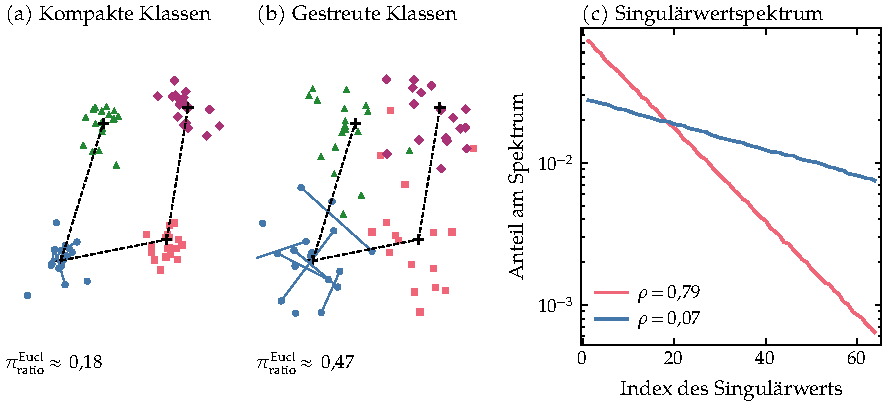
\includegraphics{neu/geometrie_konzept}
  \caption[Maße für die Geometrie eines Embedding-Raums]{Geometriemaße an synthetischen, nicht normierten Daten. (a) und (b)~Vier Klassen mit gleichen Zentren (Kreuze) und unterschiedlicher Streuung, durchgezogen: Abstände innerhalb einer Klasse, gestrichelt: Abstände zwischen Zentren, $\pi_{\mathrm{ratio}}^{\mathrm{Eucl}}$: euklidisches Gegenstück zum Maß aus Gleichung~\eqref{eq:piratio}. (c)~Normierte Singulärwerte zweier 64-dimensionaler Matrizen mit wenigen (rot) und vielen (blau) genutzten Richtungen mit ihrem spektralen Abfall $\rho$. Maße nach~\cite{roth_revisiting_2020}.}
  \label{fig:geometrie:konzept}
\end{figure}

Gemeinsam beschreiben diese Maße, wie stark ein Training den Raum komprimiert und wie weit die Klassen im Verhältnis zu ihrem Abstand streuen~\cite{roth_revisiting_2020}. Kapitel~\ref{chap:ergebnisse} verwendet sie, um die Wirkung der semi-supervised Verfahren über den Trainingsverlauf zu verfolgen.

\section{Vision Transformer und DINOv2}
\label{sec:vit}

Ein \ac{ViT} überträgt die aus der Sprachverarbeitung stammende Transformer-Architektur \cite{vaswani_attention_2017} auf Bilder \cite{dosovitskiy_image_2020}. Seine Eingabe ist eine Folge aus einem zusätzlichen lernbaren \aclu{CLS}-Token (\acs{CLS}-Token) und je einem linear projizierten, positionskodierten Vektor für jeden nicht überlappenden Patch fester Größe. Die Eingabe durchläuft mehrere Transformer-Blöcke mit Self-Attention. Klassifiziert wird anschließend allein anhand des Ausgangs an der Position des \ac{CLS}-Tokens~\cite{dosovitskiy_image_2020}.



DINOv2 bezeichnet eine Familie von \acp{ViT}, die ohne Labels auf einer kuratierten Sammlung von 142 Millionen Bildern (LVD-142M) vortrainiert werden. Das self-supervised Trainingsverfahren basiert dabei unter anderem auf einer Selbstdistillation zwischen einem Student- und einem Teacher-Netz. Als Teacher bei der Destillation des hier verwendeten ViT-B/14 diente das ViT-g. Das ViT-B/14 arbeitet mit Patches zu je $14\times14$ Pixeln und einer Embedding-Dimension von 768 \cite{oquab_dinov2_2023}. Entsprechend ist auch der Ausgabevektor des \ac{CLS}-Tokens, hier die globale Bildrepräsentation, 768-dimensional.

 
Für die Auswertung ist die Zusammensetzung der Vortrainingsdaten wichtig. Bei der Erstellung von LVD-142M dienten unter anderem die ursprünglichen Klassifikations-Trainingssplits von Stanford Cars und \ac{CUB} als Ausgangspunkt für die Auswahl von Webbildern. Über eine clusterbasierte Suche wurden für jeden der beiden Datensätze jeweils eine Million Webbilder aufgenommen~\cite{oquab_dinov2_2023}.

In-Shop und Semi-iNat-2021 dienten nicht als Ausgangsdatensätze dieser Auswahl. Ein linearer Klassifikator auf den eingefrorenen DINOv2-Merkmalen trennt die Klassen von Stanford Cars fast so gut wie die von \ac{CUB}~\cite{oquab_dinov2_2023}.

Für diese Arbeit folgt daraus, dass die Referenzdatensätze für die Auswahl der Vortrainingsbilder auch Bilder jener Automodelle und jener Vogelarten umfassten, die im \ac{DML}-Protokoll als ungesehene Testklassen gelten. Bei Cars196 verteilt der ursprüngliche Split die Bilder jeder Klasse etwa zur Hälfte auf Training und Test~\cite{krause_3d_2013}. Bei \ac{CUB} enthält der offizielle Trainingssplit nach Prüfung seiner Split-Datei in dieser Arbeit ebenfalls Bilder aller 200 Arten \cite{oquab_dinov2_2023}.

Die DINOv2-Modelle werden vor allem anhand ihrer eingefrorenen Merkmale bewertet. Dazu werden lineare Klassifikatoren auf diesen Merkmalen trainiert oder Nearest-Neighbor-Verfahren eingesetzt~\cite{oquab_dinov2_2023}. In dieser Arbeit wird das Backbone eingefroren und nur ein linearer Head mit anschließender Normierung trainiert. Nach Gleichung~\eqref{eq:mahalanobis} lernt das Verfahren damit eine Mahalanobis-artige Gewichtung der vortrainierten Merkmale \cite{weinberger_distance_2009}. Die Verlustfunktionen, das Sampling und das Evaluationsprotokoll übernimmt die Arbeit dennoch aus dem \ac{DML}.

\section{Modellauswahl und Hyperparameteroptimierung}
\label{sec:modellauswahl}

Jedes Trainingsverfahren hat Hyperparameter wie die Lernrate, die Batchgröße oder die Parameter der Verlustfunktion, von deren Werten oft abhängt, wie gut das trainierte Modell wird~\cite{bischl_hyperparameter_2023}. Gewählt werden sie beispielsweise anhand einer Schätzung des Generalisierungsfehlers auf \emph{Validierungsdaten}, die nicht zum Training gehören. Wird dabei der beste Validierungswert selbst als Leistung berichtet, ist diese Schätzung zu optimistisch, weshalb die abschließende Schätzung Testdaten braucht, die in die Auswahl nicht eingegangen sind~\cite{bischl_hyperparameter_2023}. Dasselbe gilt für den Zeitpunkt, zu dem das Training beendet wird~\cite{musgrave_metric_2020}. Beim \emph{Early Stopping} entscheidet deshalb die Validierungsleistung sowohl über das Ende des Trainings als auch über die Epoche, deren Modell getestet wird. Eine Studie zum Training von Retrieval-Modellen beendet es nach einer festen Zahl von Epochen ohne Verbesserung~\cite{berton_all_2025}, die diese Arbeit als \emph{Patience} bezeichnet.

Nach \textcite{musgrave_metric_2020} beruhen viele berichtete Fortschritte des \ac{DML} auf Unterschieden im Versuchsaufbau, etwa auf verschiedenen Backbones, Embedding-Größen und Vorverarbeitungen. Aus Versuchen, in denen die Batchgröße, die Vorverarbeitung, die Architektur und die Embedding-Dimension einzeln variiert werden, folgern auch \textcite{roth_revisiting_2020}, dass schon die Wahl dieser Größen die Ergebnisse stark verschieben kann. Weil die übliche Aufteilung nur Trainings- und Testklassen vorsieht, ist zudem der in den meisten Arbeiten berichtete Testwert zugleich der Wert, nach dem Hyperparameter und Trainingsdauer gewählt wurden~\cite{musgrave_metric_2020}. Die Validierung sollte im \ac{DML} deshalb auf Klassen erfolgen, die nicht für das Training verwendet wurden.

Die \emph{klassendisjunkte Kreuzvalidierung} teilt die Trainingsklassen in $n_{\mathrm{F}}$ Folds, trainiert für jeden Fold ein Modell auf den übrigen Folds und validiert es auf den Klassen des ausgelassenen Folds, wobei der Mittelwert dieser Validierungen die Hyperparametersuche leitet~\cite{musgrave_metric_2020}. Anschließend werden die $n_{\mathrm{F}}$ Modelle dort auf den Testklassen bewertet, einzeln und mit verketteten Embeddings. Abschnitt~\ref{sec:protokoll} beschreibt die Umsetzung in dieser Arbeit.

Bei der beschriebenen Kreuzvalidierung bleiben die Testklassen je Datensatz fest. Der Benchmark ooDML prüft Verfahren dagegen neben der üblichen Aufteilung auf weiteren klassendisjunkten Aufteilungen, deren Trainings- und Testbilder unterschiedlich stark voneinander abweichen, gemessen mit einer Fréchet-Distanz auf den Merkmalen eines ResNet50-Klassifikators. Die stärker verschobenen Aufteilungen, die dort durch den Tausch ganzer Klassen zwischen Training und Test und zuletzt durch das Entfernen weiterer Klassen entstehen, senken die Recall@1 aller untersuchten Verfahren \cite{milbich_characterizing_2021}. 

Es gibt eine Reihe von Suchverfahren, von der Gittersuche und der zufälligen Suche bis zur Bayes'schen Optimierung \cite{bischl_hyperparameter_2023}. 
Da häufig nur wenige Hyperparameter die Leistung stark beeinflussen,
untersucht eine zufällige Suche bei gleicher Zahl von Versuchen
typischerweise mehr unterschiedliche Werte dieser Hyperparameter
als eine Gittersuche \cite{bergstra_random_2012}.
Modellbasierte Verfahren berücksichtigen dagegen die Ergebnisse
bisheriger Versuche, um gezielt neue Konfigurationen auszuwählen
\cite{bischl_hyperparameter_2023}. Der \ac{TPE} teilt dazu die bisherigen Konfigurationen anhand eines Quantils der beobachteten Zielwerte in bessere und übrige, schätzt für beide Gruppen eine eigene Dichte und bevorzugt neue Konfigurationen mit einem hohen Verhältnis der ersten zur zweiten Dichte~\cite{bergstra_algorithms_2011}. Während die ursprüngliche Variante für jeden Hyperparameter eine eigene eindimensionale Dichte schätzt, modelliert die multivariate Variante die Hyperparameter gemeinsam und kann dadurch Abhängigkeiten zwischen ihnen berücksichtigen~\cite{watanabe_tree-structured_2023}.


Für die Frage, welche Hyperparameter die Leistung überhaupt beeinflussen, verwendet diese Arbeit nur die zufälligen Versuche, denn Effektschätzungen, die ein Ersatzmodell aus den Versuchen einer Bayes'schen Optimierung ableitet, können durch deren ungleichmäßige Abtastung des Suchraums verzerrt sein~\cite{moosbauer_explaining_2021}. Liegen viele Konfigurationen innerhalb der Messunsicherheit des besten Versuchs, wird in dieser Arbeit nicht der genaue Wert der gewählten Konfiguration gedeutet, sondern nur der Bereich, in dem gute Werte liegen. Ein ähnlicher Gedanke liegt der Ein-Standardfehler-Regel zugrunde, bei der neben der Validierungsleistung auch die Einfachheit des Modells berücksichtigt wird~\cite{bischl_hyperparameter_2023}.



